\documentclass[12pt,tikz]{standalone}
 
\usepackage{tkz-euclide}
\usetikzlibrary{shapes,backgrounds}
 
\begin{document}
		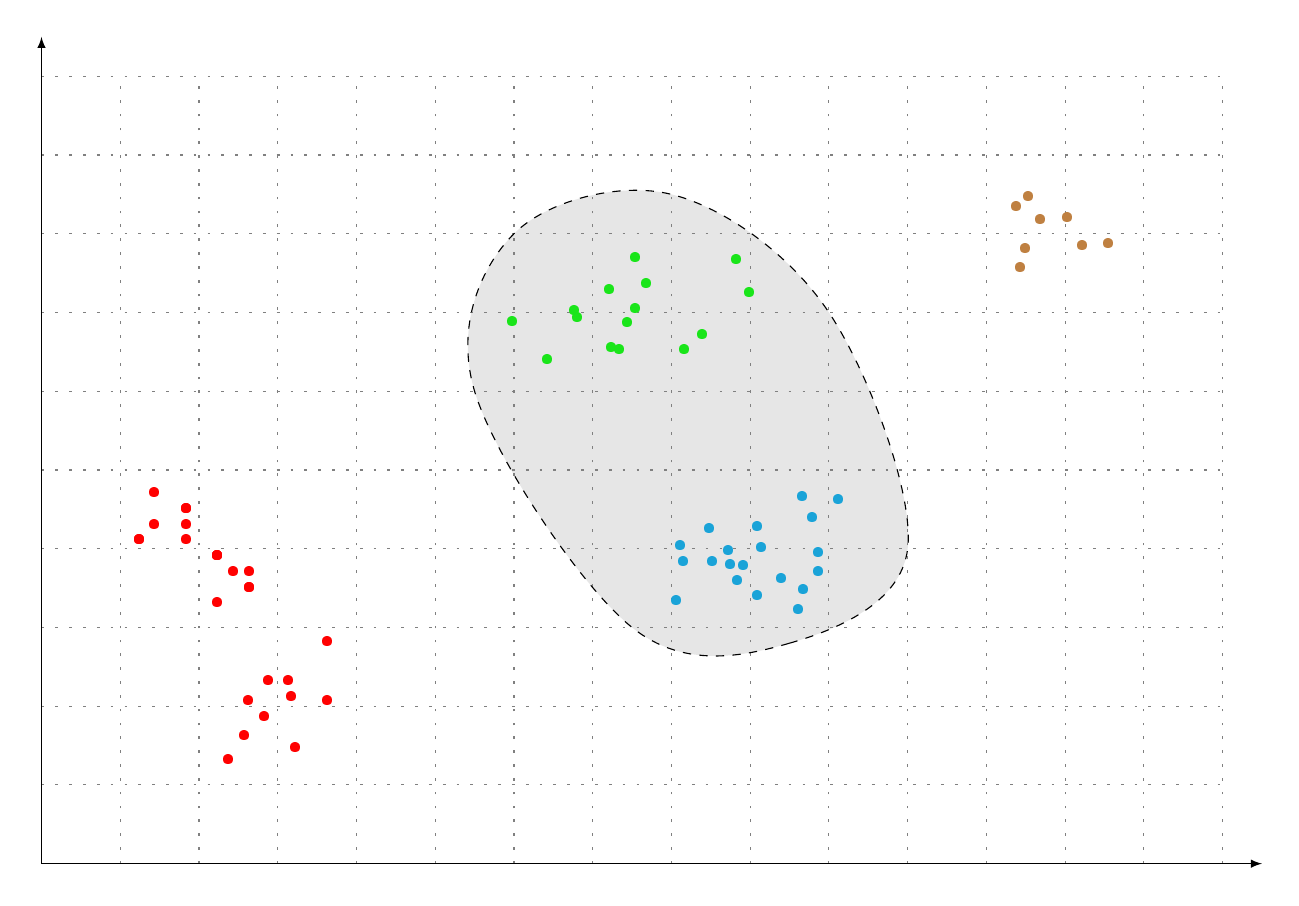
\begin{tikzpicture}[scale=1]
		   \tkzInit[xmax=15,ymax=10,xmin=0,ymin=0]
			\begin{scope}[dash pattern=on 1pt off 4pt]
			\tkzGrid
			\end{scope}
		   \tkzLabelX[orig=true,label options={font=\normalfont},step=1]
		   \tkzLabelY[orig=false,label options={font=\normalfont}]
		   \tkzDrawX[label={}] %right space=1.0,
		   \tkzDrawY[label={}]
%		   \tkzAxeXY
			% red cluster 1
			\begin{scope}[shift={(3,2)}]
				\node [red] at ( 0.13,  0.31) {\textbullet};
				\node [red] at ( 0.63,  0.81) {\textbullet};
				\node [red] at (-0.12,  0.31) {\textbullet};
				\node [red] at ( 0.63,  0.06) {\textbullet};
				\node [red] at ( 0.23, -0.54) {\textbullet};
				\node [red] at (-0.42, -0.39) {\textbullet};
				\node [red] at (-0.37,  0.06) {\textbullet};
				\node [red] at (-0.62, -0.69) {\textbullet};
				\node [red] at ( 0.18,  0.11) {\textbullet};
				\node [red] at (-0.17, -0.14) {\textbullet};
			\end{scope}
			% blue cluster 2
			\begin{scope}[shift = {(2,4)}]
				\node [red] at (-0.7625,  0.1 ) {\textbullet};
				\node [red] at (-0.1625,  0.5 ) {\textbullet};
				\node [red] at (-0.5625,  0.7 ) {\textbullet};
				\node [red] at (-0.5625,  0.3 ) {\textbullet};
				\node [red] at (-0.1625,  0.3 ) {\textbullet};
				\node [red] at (-0.7625,  0.1 ) {\textbullet};
				\node [red] at (-0.1625,  0.5 ) {\textbullet};
				\node [red] at (-0.1625,  0.1 ) {\textbullet};
				\node [red] at ( 0.2375, -0.1 ) {\textbullet};
				\node [red] at ( 0.6375, -0.5 ) {\textbullet};
				\node [red] at ( 0.6375, -0.3 ) {\textbullet};
				\node [red] at ( 0.2375, -0.1 ) {\textbullet};
				\node [red] at ( 0.2375, -0.7 ) {\textbullet};
				\node [red] at ( 0.6375, -0.5 ) {\textbullet};
				\node [red] at ( 0.4375, -0.3 ) {\textbullet};
				\node [red] at ( 0.2375, -0.1 ) {\textbullet};
			\end{scope}

			% green cluster 3
			\begin{scope}[shift = {(8,7)}]
				\node [green] at (-1.187942  , -0.08078727) {\textbullet};
				\node [green] at (-2.01881259, -0.12232100) {\textbullet};
				\node [green] at (-0.45452847,  0.69115468) {\textbullet};
				\node [green] at ( 0.9967442,  0.24416339)  {\textbullet};
				\node [green] at ( 0.16518064, -0.47996454) {\textbullet};
				\node [green] at (-0.78641819,  0.27659986) {\textbullet};
				\node [green] at (-0.7684694 , -0.45329367) {\textbullet};
				\node [green] at ( 0.39634632, -0.29201342) {\textbullet};
				\node [green] at ( 0.82322753,  0.65666408) {\textbullet};
				\node [green] at (-0.3204896 ,  0.35999170) {\textbullet};
				\node [green] at (-0.45671327,  0.03756002) {\textbullet};
				\node [green] at (-0.56043534, -0.14037135) {\textbullet};
				\node [green] at (-1.57446398, -0.61435168) {\textbullet};
				\node [green] at (-0.66513607, -0.48349494) {\textbullet};
				\node [green] at (-1.23802023,  0.01343445) {\textbullet};
			\end{scope}
			% cyan cluster 4
			\begin{scope}[shift= {(9,4)}, scale=0.6]
				\node [cyan] at ( 1.44732954, -0.10426899) {\textbullet};
				\node [cyan] at ( 0.14345684,  0.46001939) {\textbullet};
				\node [cyan] at (-0.13311515, -0.36526611) {\textbullet};
				\node [cyan] at (-1.40244442, -0.29656337) {\textbullet};
				\node [cyan] at (-0.80883943, -0.28461161) {\textbullet};
				\node [cyan] at ( 1.31343245,  0.63835941) {\textbullet};
				\node [cyan] at ( 0.15882059, -1.01732324) {\textbullet};
				\node [cyan] at (-1.55368128, -1.10825507) {\textbullet};
				\node [cyan] at ( 0.24811186, -0.00462673) {\textbullet};
				\node [cyan] at ( 1.86304926,  1.02213552) {\textbullet};
				\node [cyan] at ( 0.65681417, -0.64120414) {\textbullet};
				\node [cyan] at (-0.41631369, -0.35833488) {\textbullet};
				\node [cyan] at ( 1.44421909, -0.50605346) {\textbullet};
				\node [cyan] at (-0.45642586, -0.05247862) {\textbullet};
				\node [cyan] at (-1.48646435,  0.05521688) {\textbullet};
				\node [cyan] at ( 1.09558337,  1.086727  ) {\textbullet};
				\node [cyan] at ( 1.12190388, -0.89123234) {\textbullet};
				\node [cyan] at (-.85727929,  0.40846484) {\textbullet};
				\node [cyan] at ( 1.02101185, -1.31617783) {\textbullet};
				\node [cyan] at (-0.26372957, -0.69867008) {\textbullet};
			\end{scope}
			\draw [black, fill=white!50!black, fill opacity=0.2, shift={(0,1)}, dash pattern=on 3pt off 3pt] plot [smooth cycle,tension=0.6] coordinates {
				(7.5, 2) (9.5, 1.8) (11,3) (10,6) (8,7.5) (6,7) (5.5,5)
			};
			% brown cluster 5
			\begin{scope}[shift={(13,8)}, scale=0.5]
				\node [brown] at (-0.99859068, -0.39862533) {\textbullet};
				\node [brown] at (-0.93951106,  0.91323855) {\textbullet};
				\node [brown] at ( 0.06707937,  0.38156436) {\textbullet};
				\node [brown] at (-1.24353468,  0.66339294) {\textbullet};
				\node [brown] at (-1.12527052, -0.87136462) {\textbullet};
				\node [brown] at ( 0.43065155, -0.33411968) {\textbullet};
				\node [brown] at ( 1.08696849, -0.26349634) {\textbullet};
				\node [brown] at (-0.61973447,  0.34853987) {\textbullet};
			\end{scope}		
		\end{tikzpicture}
\end{document}